\renewcommand{\theequation}{\theenumi}
\begin{enumerate}[label=\thesection.\arabic*.,ref=\thesection.\theenumi]
\numberwithin{equation}{enumi}

\item Draw Fig. \ref{fig:eq1}, \ref{fig:eq2}, \ref{fig:eq3}, \ref{fig:eq4}, \ref{fig:eq5} .\\

\solution The  following Python code generates all the figures.
\begin{lstlisting}
codes/linear_eq_roots.py
\end{lstlisting}

\begin{figure}[h!]
\centering
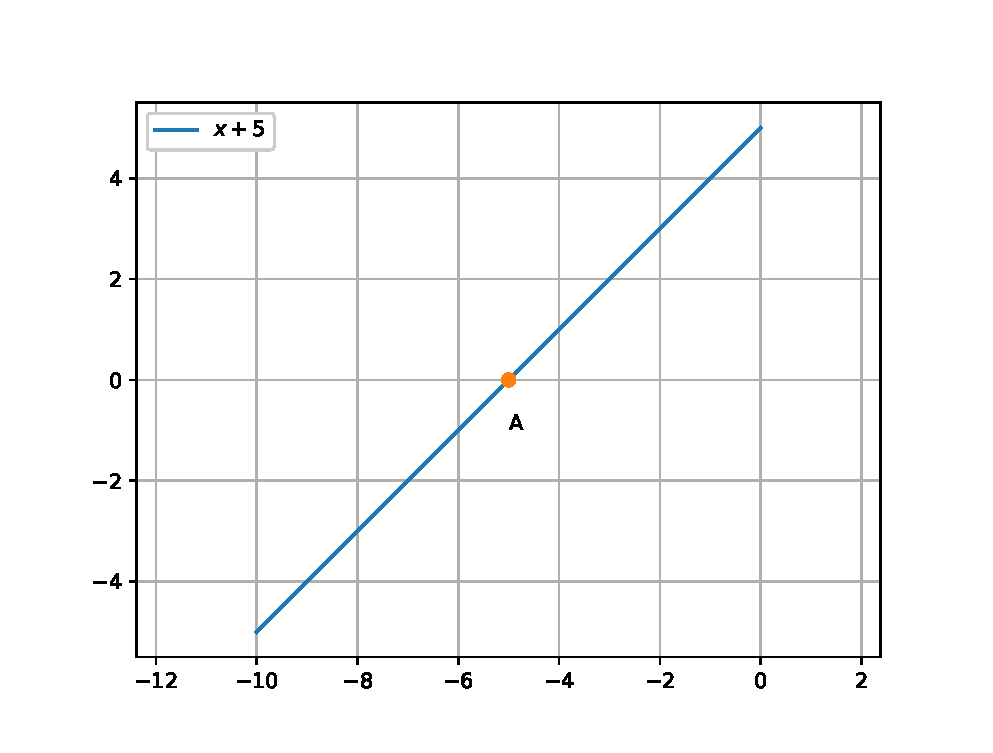
\includegraphics[width=\columnwidth]{./figs/eq1.eps}
\caption{$x + 5$ generated using python}
\label{fig:eq1}
\end{figure} 

\begin{figure}[h!]
\centering
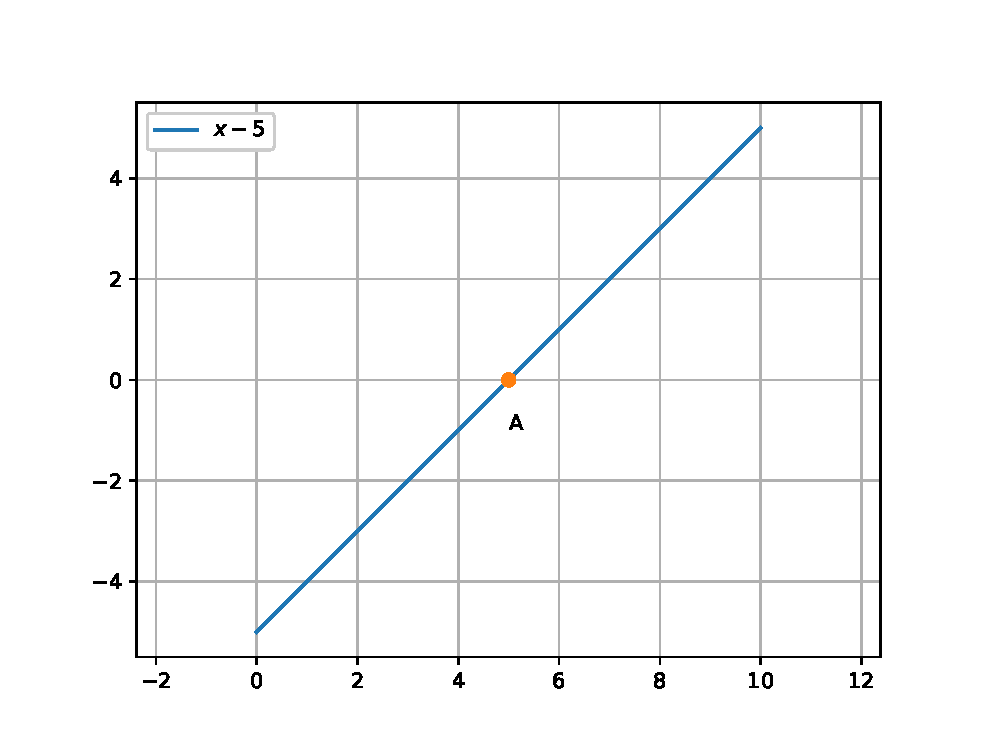
\includegraphics[width=\columnwidth]{./figs/eq2.eps}
\caption{$x - 5$ generated using python}
\label{fig:eq2}
\end{figure} 

\begin{figure}[h!]
\centering
\includegraphics[width=\columnwidth]{./figs/eq3.eps}
\caption{$2x + 5$ generated using python}
\label{fig:eq3}
\end{figure} 

\begin{figure}[h!]
\centering
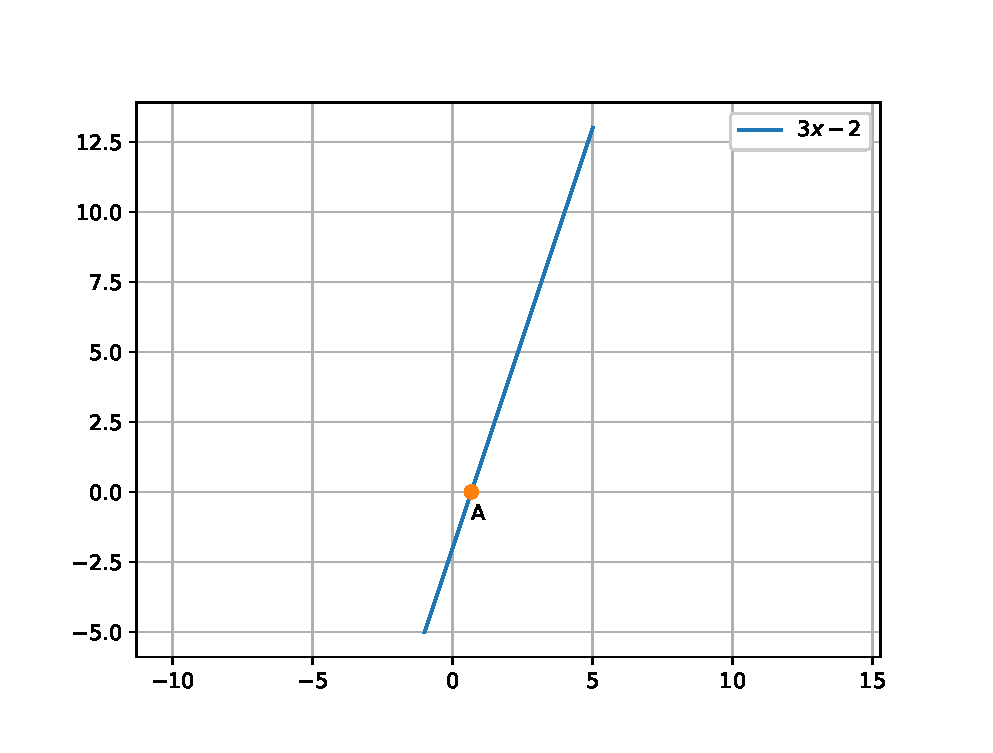
\includegraphics[width=\columnwidth]{./figs/eq4.eps}
\caption{$3x - 2$ generated using python}
\label{fig:eq4}
\end{figure} 

\begin{figure}[h!]
\centering
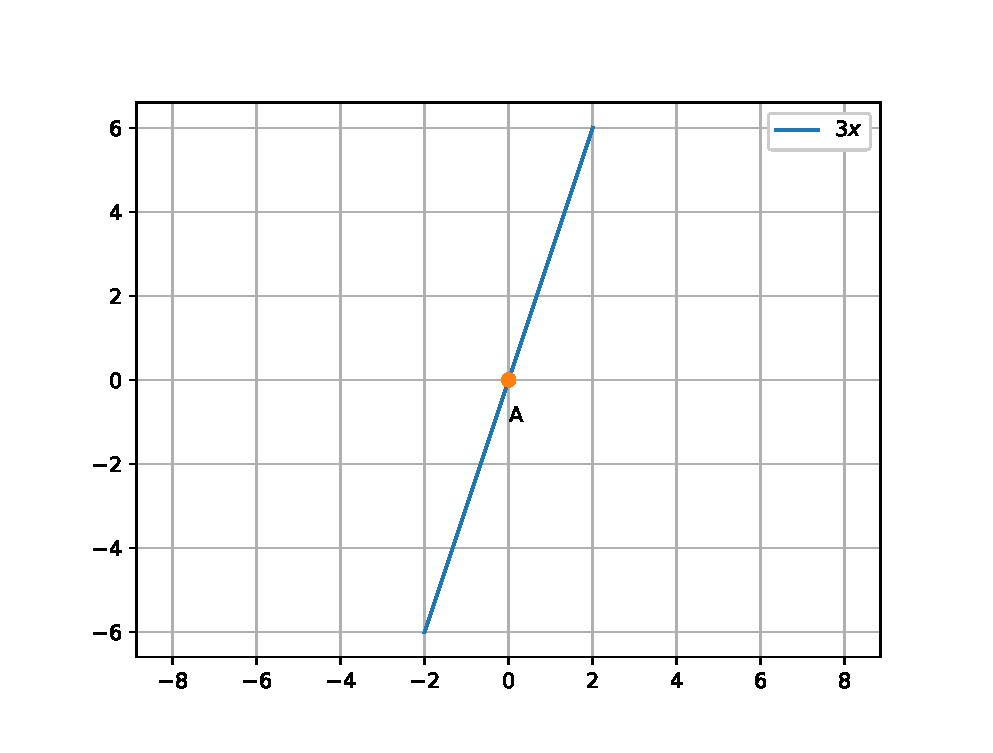
\includegraphics[width=\columnwidth]{./figs/eq5.eps}
\caption{$3x$ generated using python}
\label{fig:eq5}
\end{figure} 


\end{enumerate}
